\red{\textbf{COMPLETE THIS SECTION LAST}

The Executive Summary offers a succinct statement of your findings and contributions.

It will summarise the project description and your contributions to the associated discipline.  

This section can be based on key sentences and paragraphs from your Scope of Works and Progress Report documents, and your Conclusions and Recommendations section.

No more than five pages of text and images.

Introduction section begins the story of your project.  Include a clear statement of objectives and the scope of the project (the Scope of Works document can be used as a basis). Your report can then begin with the starting point of the project – the “need” or “want”. \\

WHAT DOES OUR AIRCRAFT BRING TO THE RESEARCH COMMUNITY:
\begin{itemize}
	\item Low cost autonomous aircraft (compare to Sony, defence drones, DJI and Parrot)
	\item Hybrid aircraft with transition capability (novel flight capabilities)
	\item Long range AND long flight time in a single unit (best of both aircraft)
	\item Foundations for intelligent drone flight (not just ``follow me'' behaviour)
	\item Uncountable applications beyond medical transport (list)
\end{itemize}}
\todo{finish this and use the sections as a guide}
\subsection{Objectives and Scope}
\subsection{Context}
The UAV Challenge \cite{ref:challenge}, organised by the Queensland University of Technology and the CSIRO, is a biennial competition that aims to push the boundaries of current autonomous aircraft technology. The 2016 challenge is titled ``Medical Express'', and charges teams with solving the issues raised above.\\

Competitors must develop an aircraft that can fly to a known area (up to 30km away) through specific transit corridors, search for and correctly identify ``Outback Joe'', land close to him in an obstacle-rich environment, accept a pre-prepared blood sample, and then fly back to base. All of these actions must be completed within one hour, and must be fully autonomous; that is, after receiving the ``start'' signal the aircraft must have no human input.

\subsection{Project Outline}
This project involves the development of an autonomous Unmanned Aerial Vehicle (UAV) with the capabilities to compete in the 2016 UAV Challenge. Given the Challenge specifications above, a number of design and performance requirements were identified that aircraft must meet in order to be successful:
\begin{enumerate}[label=\bfseries R\arabic*:] \itemsep-2pt
	\item Aircraft must be autonomous
	\item Take-off and landing in obstacle-rich environments (i.e. without a runway)
	\item Total flight endurance of at least 60km
	\item Total flight duration of up to 60 minutes
	\item Automated in-flight identification of a known target
	\item Ability to receive 500g payload upon landing
\end{enumerate}

It is anticipated that there will be several Capstone student teams continuing development of the UAV in 2016. Given the requirements listed above, and the timeline of the Challenge, the \ID project team sought to develop a working prototype with which to achieve the basic functionality required to compete in the Challenge. As such, the following objectives were selected for the project:
\begin{enumerate}[label=\bfseries O\arabic*:] \itemsep-2pt
	\item Register for the 2016 UAV Challenge
	\item Development of a prototype UAV for future teams to build on
	\item Development of autonomous flight controls to achieve \textbf{R1}
	\item Development of a novel hybrid flight system, incorporating both Vertical Take-Off and Landing (VTOL) and Fixed-Wing flight modes, for future teams to build upon to achieve requirements \textbf{R2}, \textbf{R3} and \textbf{R4}
	\item Development of in-flight search and obstacle avoidance mechanisms to be able to achieve \textbf{R5}
\end{enumerate}

The remaining sections of the report will discuss the work conducted by \ID in developing a working prototype for the UAV Challenge, beginning with a brief review of existing approaches that motivated the design of the UAV developed in this project. The following sections will discuss the various development domains of the UAV, including its design, flight and planning systems, and sensing systems, with a particular focus on the novel transition system developed for hybrid flight. The report will end with the results achieved by team \ID, work to be completed, and recommendations for 2016 teams in continuing the UAV's development.

\subsection{Key Findings}
\subsubsection*{Proposed Design}
The initial prototype design for this project will use a PixHawk flight controller in a Skywalker X8 airframe, mounted with three motors in a tri-coptor configuration. The aircraft will also be fitted with a transition system, to rotate the front motors and enable the aircraft to fly in both VTOL and fixed-wing modes. Finally, the aircraft will be mounted with various sensors, discussed in Section \ref{sec:sensing}, including a camera and LiDAR, to provide sensing capabilities for planning, obstacle detection and autonomous flight.\\

Figure \ref{fig:hardwarearch} shows a high level overview of the hardware architecture planned for the current and future teams.

\begin{figure}[!h]
	\centering
	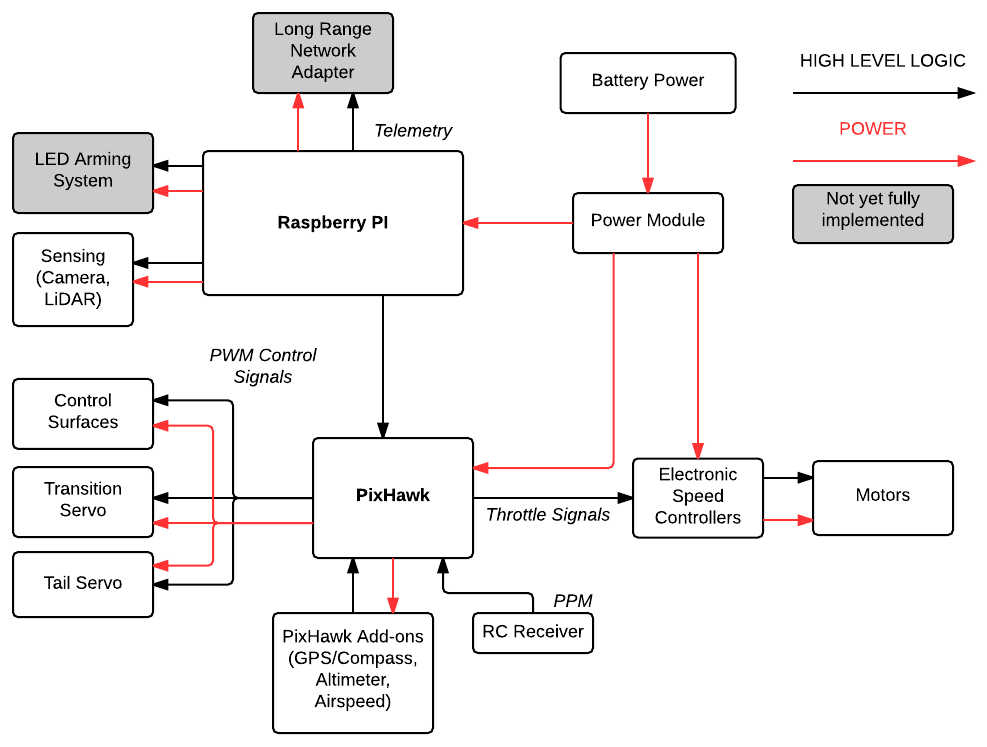
\includegraphics[width=380pt]{\IMAGEPATH /Diagrams/hardware}
	\caption{High level hardware architecture}
	\label{fig:hardwarearch}
\end{figure}

\subsection{Why Transition?}
In order for the UAV to complete the objectives listed previously, it must be capable of both long range flight and vertical take-off and landing. Implementing a transition system, rather than fit the UAV with both fixed-wing and VTOL flight systems, allows it to achieve this capability while also being lighter, and more aerodynamic. The transition systems is the foundation for achieving the range and endurance requirements of the UAV Challenge.

\subsection{Design}
- basic outcome
\subsection{Sensors and Autonomy}
- basic outcome
\subsection{Achievements, conclusion and recommendations}